\section{Introduction}
In the context of the personal project course given at ULiège. I decided to develop a smart freezer. This idea emerges due do a personal experience. Every year my family and I reorganize the home's freezers. I was a bit shocked when I saw the quantity of products that were in the freezers and for which I was not aware. This is a problem that anyone can potentially face one day. \\

The main problem of forgotten products is they cannot stay indefinitely to a freezer due to they physical properties. For instance after some time a meat staying for a long time into a freezer will not have a good taste. As results, some products were thrown to the rubbish. We could avoid to throw to the rubbish products if we are aware of the existence of that products. The solution of that problem would be an application or a tool that gives the possibility to manage the content of your freezers and more. It is the direction that I took for my personal project.

\subsection{Explanation of the project itself}
The project consists of an application that will give you some information about the products stored into the user's freezers. The period since a product is stored into a specific freezer. Each product will be linked to a unique user due to the fact that most of the products stored in a freezer are \textit{home-made products}. This means that a same product cannot be shared with two different people.\\

The application gives the possibility to directly find what you want with a specific nomenclature. Each product has a serial number by box and by freezer (if the user has several freezers). Each time a product comes in/out of the freezer the user needs to notify this manipulation to the application.\\

Moreover, the application has the possibility to do suggestions to the user according to his previous consumption and depending on what his / her freezer(s) contain for some time. The goal being that the application helps the user in his choices and also remind him what he has in his freezer and what should perhaps be consumed in first. \\

For this project the application is restricted to a web application but can be easily ported to others terminals due to the fact that the back-end part is based on a REST API which is cross-platform.

Front-end part and back-end part a aborder
\section{Content storing}
\subsection{Database model discussion}
To store the different information about a user and the data related to his freezers a database is required. There exists several types of databases and it is no so easy to make a choice that will not have bad impacts on the future if the choice made at the beginning was not good. The choice made is a relational database. this choice is motivated by several things. First of all, the problem is known and I know the links to establish between data. Moreover, data would not change on the long-term which means that the architecture of the database would not change a lot and the quantity of information to store will never be huge. Finally, data to store is essentially texts and numbers, thus no need to have a database that can manage video streams etc like noSQL database.\\

The relational database management system chosen is MySQL since it is an open-source software which is commonly use.
\subsection{Relational database structure}
The information that the database need to store will be explained in detailed.\\

First of all, we need to store some information about a user such as an email and a password that allow the user to establish a connection with the main website. This website gives additional information about the user such as the token linked to the user account. This token is mandatory to have access to the API used to manage his freezers. A user has also two additional information which are the language and learning fields. The language field is used to specify the language used by the user. It can be interesting for third applications to have some knowledge about the user. The learning is used to save some parameters that could be useful for learning algorithm. For this project I do no use it because I did not have enough time to find and test some of these. \\

The database contains several types of products. These types of products can only be added by the administrator of the system. A product type is described by an identification a name given in English and a name given in French. \\

The users's freezers should be described by the user. A freezer is descried with three elements . The first one is a unique identifier to be identified into the database. This parameter is automatically done by the system itself, the user does not need to manage this parameter. The two other parameters are the number of boxes that the freezer contains and the second one is the name given by the user to the freezer. \\

A freezer product from a user contains several fields. First of all, a unique identifier given by the system itself. A date of input, this date must be anterior to the date of its entrance in the freezer. In other words it is impossible to encode product with a date that refers to a place in the future. A date of output, by default this field is set to null. when this field is not null it means that the product is not any more in the freezer. The date of output must be greater or equal to the date of input. A product also contains a period field which is used to define the period in months for which the product should be in the freezer. Then third applications can display products that overcome this period. The quantity is also a piece of information of a product. It gives  the quantity in terms of person for which the product can be used. Finally, a product also have two additional fields to allow a user to locate more easily a product. These two additional fields are the box number which give the box for a specific freezer and the product identifier which allows to locate the product in this box. This identifier is unique for the specific box. \\

A product also receives a description . The product description contains three different fields which are the description identifier, the product name and a free description of the product. This description can be a structured description or a simple text. \\

\subsection{Entity-relationship model}
The \autoref{fig:reldb} shows the entity-relationship model of the freezer database. As we can see on this schema the relations \textit{list\_freezer} and \textit{product\_to\_type} are not mandatory since the information that they linked can be retrieved from the rest of the database. These two relations have been inserted into the database for a simplicity since these information are often asked. Knowing that it is interesting for the backup part. \\

\begin{figure}[H]
\centering
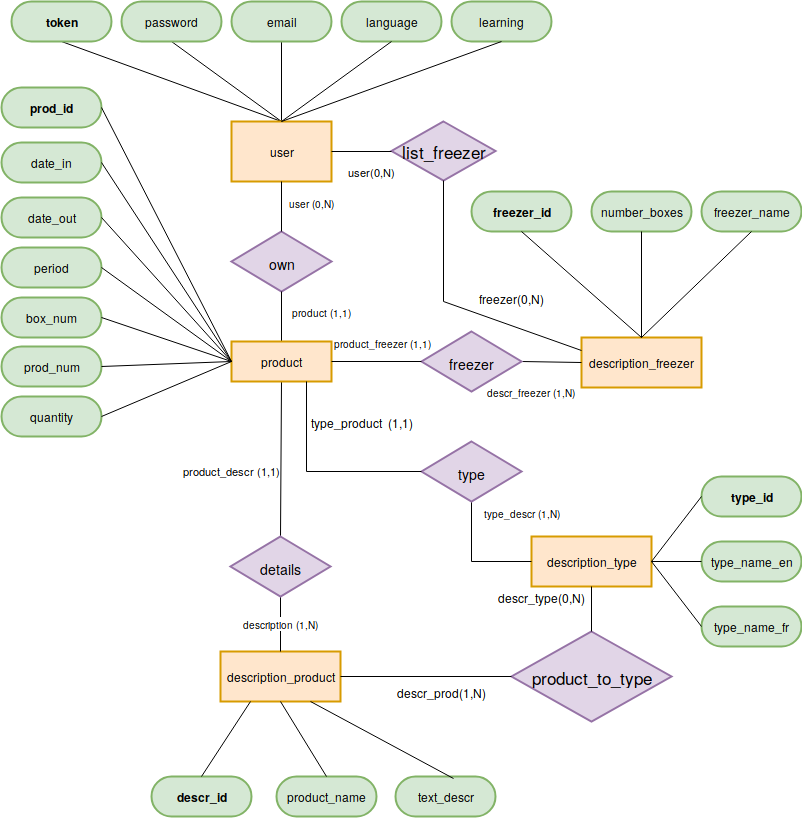
\includegraphics[scale=0.5]{./images/reldb.png}
\caption{entity-relationship model of the database}
\label{fig:reldb}
\end{figure}

\subsection{Relational model}
From the entity-relationship we can go into the relational format which allow to have a representation for integrating the database into a relational database management system.
\begin{enumerate}
\item User(\underline{\textbf{token}}, password, \underline{email}, language, learning)
\item Description\_type(\underline{\textbf{type\_id}}, type\_name\_en , type\_name\_fr)
\item Description\_product(\underline{\textbf{descr\_id}}, product\_name, text\_descr)
\item Description\_freezer(\underline{\textbf{freezer\_id}}, number\_boxes, freezer\_name)
\item Product\_to\_type(\textbf{\#descr\_id, \#type\_id})
\item List\_freezers(\textbf{\#freezer\_id, \#token})
\item Product(\underline{\textbf{prod\_id}}, \#token, \#descr\_id, \#freezer\_id, \#type\_id, date\_in, date\_out, period, box\_num, prod\_num, quantity)
\end{enumerate}

The database is encoded in MySQL language. The engine used is InnoDB with utf8mb4\_unicode\_ci as collation. The choice of this engine has been done because is the default engine and manage ACID transactions and foreign keys. The \autoref{fig:sqldb} depicts the MySQL implemented and the types associated to each variable. The choices made for the length size of variables are personal choices. But the length size can be changed with no difficulties if the need arose. The encoding chosen allows to be flexible as much as possible.

\begin{figure}[H]
\centering
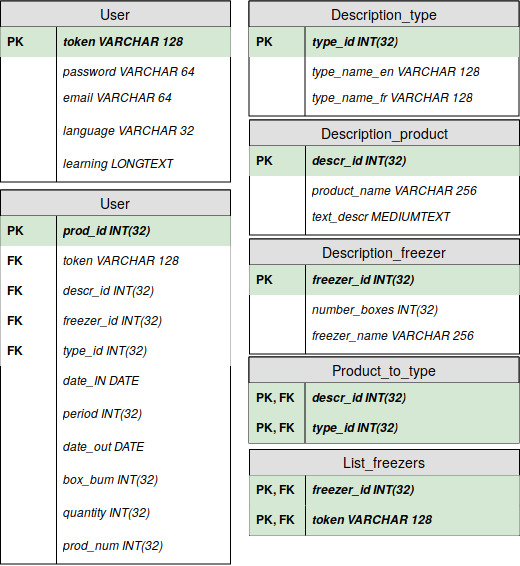
\includegraphics[scale=0.5]{./images/sqldb.jpg}
\caption{slq tables of the database}
\label{fig:sqldb}
\end{figure}

As discussed above the architecture of the database allows to skip some tables to backup like Product\_to\_type and List\_freezers. These two table can be reconstruct with the others tables. Thus it is not mandatory to backups these ones.

\subsection{Account creation}
To use the API a user need to create an account with an e-mail address and a password. A webpage is built to achieve this goal( \textit{register.php}). When the account has been created it is linked to a token. This token is generated on the server side with the PHP function \textit{random\_bytes} which is recommended to generate string of cryptographic random bytes that are suitable for cryptographic use. The length  specified for the generation is 32 bytes.Thus the number of possibilities is $(2^8)^32 = 2^256$. After that, the random sequence generated is transformed into a hexadecimal string to be more readable by a novice user.\\

When the account is created a user can use the API to build its own software and manage his freezers with the help of The API and the token linked to its account or use an existing application that uses the API. In this second case the third part application should only asked your token and anything else.\\

pourquoi choix du relationel db
mettre les schema entite relation expliquer les choix etc

 mentionner que l'encodage a été fait à la main et essentiellement pour un utilisateur -> fastidieux à faire et insérer des éléments aléatoirement n'a pas vraiment de sens du fait qu'un utilisateur n'a pas ce comportement. Ce la ne poserait pas de probleme pour la db mais c'est un travail inutile a réaliser dans l'optique du mon projet que de remplir la db avec des données aléatoire.
\section{User panel}
When a user possesses an account. He has the possibility to access to a user panel. This user panel is used to give to the user more information about its account. i.e: the email address, the token linked to the account, the possibility to change the password and the language.
Panel pour creer un compte et avoir accès à son token ainsi qu'à certaines informations relatives au fonctionnement de l'API

\section{API REST}
\subsection{Sever}
\subsection{functionalities implemented}
\subsection{Documentation}
explication des differentes fonction
 mentioner l'instoration d'une documentation détaillée et de l'utilisation 
 mentioner cORS pour prendre en compte les different domaines
 Pas de problemes pour ajouter de nouvelles fonctionnalitées ou de changer les existantes
 
 Pourquoi une API REST
 
 Mentioner l'essai du preférence learning ce qui a été fait et pas fait les probleme rencontrés etc
 \subsection{formules}

\section{Admin panel}
Pas vraiment développé
Panel qui donne acces à toute une série d'informations globales sur les utilisateurs. Pas bcp de fonctionalités pour le moment mais peut etre étendu sans problème

\section{External website}
Ce veut être une application "externe" a l'API REST et à la DB. Peut etre vu comme une société externe utilisant un service

Le but de cettte application est d'avoir une sorte de dashboard

\section{unit tests}

\section{problemes rencontrés}
\section{future work}
\section{Conclusion}
